\documentclass{article}
\usepackage[final]{neurips_2024}
\usepackage[utf8]{inputenc}
\usepackage{lmodern}
\usepackage[T1]{fontenc}
\usepackage{booktabs,multirow,amsmath,graphicx,xcolor,url,microtype,listings}
\graphicspath{{../}{./}}
\usepackage[colorlinks,linkcolor=blue!55!black,citecolor=blue!55!black,urlcolor=blue!55!black]{hyperref}
\usepackage{caption}
\captionsetup{font=small,labelfont=bf}
\lstset{basicstyle=\ttfamily\scriptsize,breaklines=true,frame=single,framesep=3pt,
        rulecolor=\color{black!25},backgroundcolor=\color{black!3},
        xleftmargin=2pt,xrightmargin=2pt,aboveskip=5pt,belowskip=3pt,columns=fullflexible}
\newcommand{\pval}[1]{$p={#1}$}

\title{Verifier-Supervised Look-Back: Label-Free Screen Retrieval for\\Delayed Information Needs in Mobile GUI Agents}
\author{Mingshuo Wang\\North Carolina State University}

\begin{document}
\maketitle
\begin{abstract}
A mobile GUI agent often has to type text it saw many screens earlier: it reads ``vanilla extract'' on a recipe page and must enter it into a shopping list nine steps later, after that screen has left the display. We call such a step a \emph{delayed information need}. The hard part is not storing the history but deciding which earlier screen to re-read, and training a model to decide it normally requires human labels. We show that no labels need to be bought. The automatic verifier used to \emph{mine} these cases (the typed text appears in the OCR of an earlier screen and not on the current one) also \emph{labels} every earlier screen as holding the text or not, at the cost of one substring test per screen. Training on those labels, which we call \emph{verifier-supervised look-back}, is what makes look-back work. It lifts a full-history reader from 54.8\% to 65.4\% source-screen localization on 188 verified cases and a per-screen scorer from 50.0\% to 72.3\%. The two trained variants are statistically indistinguishable (\pval{0.086} on localization, \pval{0.45} end-to-end), so the supervision rather than the retrieval architecture is the lever; the per-screen decomposition pays only at gaps of 8--12 screens (78.2\% vs.\ 56.4\%, \pval{0.003}). On a fourth sample of trajectories mined after every design decision was fixed and evaluated once, the two reach 79.6\% and 76.3\% against 59.1\% for prompting (\pval{0.003}), and raise end-to-end accuracy from 23.7\% to 49.5\% and 51.6\% ($p<0.001$). We also report where both trained variants fail, and two evaluation filters without which this problem cannot be measured at all.

\textbf{Code, data artifacts and all result files:} \url{https://github.com/WMSlalalala/verifier-supervised-lookback}

\end{abstract}
\section{Introduction}

\paragraph{Background.} A mobile GUI agent executes a task by repeatedly looking at a screen and emitting an action. On a long cross-app task the screens it has already seen scroll out of view, and some of them carried information it will need later. An agent that reads a recipe page, then opens a shopping list, must type ``vanilla extract'' nine steps after the only screen that ever showed those two words. We call a step whose required text appeared on an earlier screen, and only there, a \emph{delayed information need}; the screen that held the text is the \emph{source screen}, and the number of screens since is the \emph{gap}. Section~\ref{sec:needs} shows these steps are common in long tasks: 31\% of sampled GUI-Odyssey~\citep{guiodyssey} trajectories contain at least one, with a median gap of 5 screens. They are absent from the short-task benchmarks the field develops on: AITZ~\citep{aitz} has none in 18,643 steps, consistent with tasks that average 7.4 steps.

\paragraph{Existing approaches and their limitation.} Two designs recover such text, and both are prompted rather than trained. \emph{Full history} keeps the OCR text of every earlier screen in context and asks the model to name the source screen and the text in one call. \emph{Gist-and-lookup}, introduced for long documents by ReadAgent~\citep{readagent} and instantiated here as a \emph{screen index}, writes one short line per screen and asks a reader to pick a screen from the lines before re-reading it in full. Both degrade as the history grows: full history localizes the right screen in 68\% of needs that arise by step 15 and in 46\% of later ones, and the screen index reaches only 41\% overall. The shared limitation is not the representation but the supervision. Neither design has been trained for this decision, because training it means labeling which earlier screen an agent should re-read, and the one trained look-back agent we know of, PAL-UI~\citep{palui}, pays for that with 8.6K curated step-level instructions. On a new corpus, that cost is paid again.

\paragraph{The challenge.} Labeling look-back by hand is expensive for a structural reason: the label is not a property of one screen but of a relation between a step and all the screens before it, so a human annotator must read an entire trajectory to label one decision. A cheap automatic label would have to identify, for a given step, exactly which of the $t$ preceding screens could answer it. It must also be trustworthy enough to train on, which rules out heuristics such as recency or lexical overlap, both of which we show are wrong often enough to mislead a learner (Section~\ref{sec:index}).

\paragraph{Our method.} Such a label already exists, as a by-product of defining the problem. A delayed information need is verified by a string check: the typed text appears in the OCR of an earlier screen and not on the current one. Run that same check against every earlier screen rather than stopping at the first hit, and it returns the set of screens that contain the text. That set is a complete, exact label over all $t$ candidates, obtained at the cost of one substring test per screen, with no human in the loop. We call training a look-back policy on these labels \emph{verifier-supervised look-back}, and we train two instantiations on them (Figure~\ref{fig:method}): a \emph{per-screen scorer} that reads one earlier screen at a time and outputs the probability that it holds the needed text, and a \emph{full-history reader} that sees the whole history in one call and emits a screen number. A second call, the \emph{read stage}, then types the text.

\paragraph{Contributions.}
\begin{itemize}\setlength{\itemsep}{1pt}
\item \textbf{Problem and free labels.} We define delayed information needs, give an automatic verifier that both mines and labels them, and measure their prevalence: absent from AITZ, present in 31\% of sampled GUI-Odyssey trajectories (Section~\ref{sec:needs}).
\item \textbf{Method.} Verifier-supervised look-back, with two instantiations that share one label set and one objective and differ only in how the history reaches the model (Section~\ref{sec:method}).
\item \textbf{Finding: supervision, not architecture, is the lever.} The labels lift the full-history reader by 10.6 localization points and the per-screen scorer by 22.3, and reverse which architecture is better; a paired test separates the two trained variants on neither metric (Section~\ref{sec:main}). We locate the decomposition's real gain at gaps of 8--12 screens, where it is worth 21.8 points (Section~\ref{sec:gap}).
\item \textbf{External validation and honest limits.} On a fourth sample held out from every design decision, both trained variants keep a 17--20 point margin over prompting and remain indistinguishable (Section~\ref{sec:ext}). Three ablations show the design is insensitive to its prompt and loss settings (Section~\ref{sec:ablation}). At gaps of 13 or more screens both trained variants fall \emph{below} prompting, which we report rather than omit (Section~\ref{sec:limits}).
\item \textbf{Two mandatory evaluation filters.} Scoring only the earliest source screen biases one arm by 15 points, and admitting cases whose answer is also on the current screen reverses the sign of a 17-point result. We quantify both and give the filter conditions (Section~\ref{sec:index}).
\end{itemize}

\section{Method}
\label{sec:method}

\begin{figure}[t]
\centering
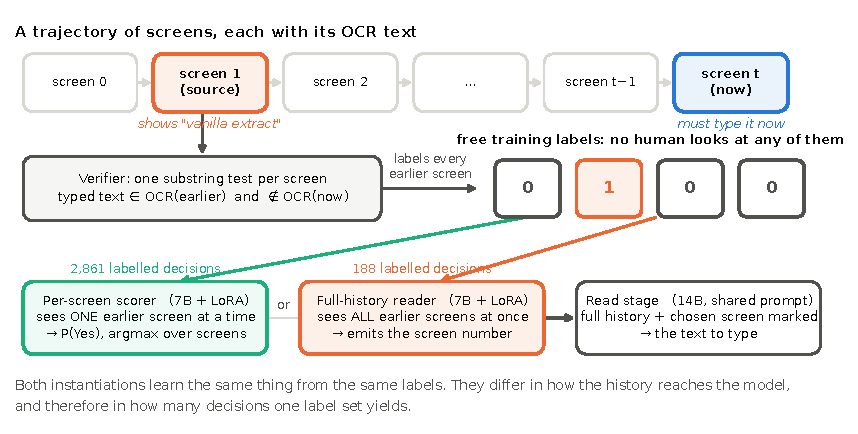
\includegraphics[width=\linewidth]{figures/fig1_method.pdf}
\caption{The verifier does two jobs. Reading left to right along the trajectory, it mines the case: the text typed at step $t$ appears in the OCR of screen 1 and not on screen $t$. Applied to every earlier screen instead of stopping at the first hit, the same test labels all $t$ candidates. Those labels train two instantiations that differ in how the history reaches the model, and therefore in how many decisions one label set yields.}
\label{fig:method}
\end{figure}

\subsection{A string check both finds and labels the needs}
\label{sec:needs}
A step $t$ has a delayed information need when the text the agent types at $t$ appears verbatim in the OCR text of an earlier screen $i<t$ and does not appear on screen $t$. The gap is $t-i$ for the latest such $i$. The second clause is load-bearing: when the text is on the current screen the agent needs no memory at all, and Section~\ref{sec:index} shows that keeping those steps rewards any method that reads recent screens.

A candidate is any TYPE action whose argument has three or more characters and does not occur in the task description; we normalize strings by lower-casing and stripping whitespace and punctuation. We run EasyOCR on every screenshot of the sampled trajectories and test the argument against earlier screens and the current one. In the first sample of 300 GUI-Odyssey trajectories, 127 of 431 candidates pass the OCR check (269 fail, most of them OCR misreads on inspection, and 35 lack OCR output). Removing 36 whose text is also on the current screen leaves 91 verified cases; removing 6 whose text appears in the task's step-by-step instruction field leaves 85. The verifier also returns the full set of screens containing the text, which is the label.

\begin{table}[t]
\centering\footnotesize\setlength{\tabcolsep}{4pt}
\caption{AITZ's 7.4-step tasks contain no delayed information need; GUI-Odyssey's 15.4-step tasks contain one in 31\% of sampled trajectories. We mine only the sampled trajectories.}
\label{tab:prev}
\resizebox{\linewidth}{!}{%
\begin{tabular}{lrrrl}
\toprule
 & trajectories & steps & mean length & verified delayed needs \\
\midrule
AITZ~\citep{aitz} & 2,504 & 18,643 & 7.4 & 0 \\
GUI-Odyssey~\citep{guiodyssey} (full) & 7,735 & 118,791 & 15.4 & not mined \\
\quad sampled, complete OCR & 273 & 4,338 & 15.9 & 89 steps (2.05\%); 31\% of trajectories \\
\bottomrule
\end{tabular}}
\end{table}

Table~\ref{tab:prev} gives the prevalence. The need is also far and inconspicuous: the gap has median 5 and maximum 27 screens, 56\% of gaps are 5 or more, and on its source screen the needed text sits at a median rank of 13 among 33 OCR elements and is never first. A one-line summary that keeps the few most prominent elements therefore cannot be expected to retain it.

\paragraph{Four samples.} The \emph{short set} holds the 85 cases above (need step index $t$, median 11). The \emph{long set} holds 53 cases with $t\ge16$ from a second sample of 300 trajectories of $\ge20$ steps (127 before the current-screen filter, all 74 removals being leakage). The \emph{late-mined set} holds 50 cases with $t\ge16$ from a third sample of 200 trajectories. These three give 188 cases in 170 trajectories and carry all training and cross-validation. The \emph{external set} holds 93 cases from a fourth sample of 400 trajectories of $\ge16$ steps, mined after every design decision was fixed and evaluated once.

\subsection{Two instantiations, one label set}
Each verified case $(e,t)$ yields one training item per earlier screen $i<t$. For the \textbf{per-screen scorer} the item is a pair: the input holds the task description, the OCR text of screen $t$, the OCR text of screen $i$ and the distance $t-i$, and the label is 1 if $i$ is in the verifier's set. The 188 cases yield 2,861 pairs, 463 of them positive. For the \textbf{full-history reader} the item is one example per case: the input holds the task and every earlier screen, and the target is the number of the latest screen in the verifier's set. No human labels any item.

The scorer is Qwen2.5-7B-Instruct~\citep{qwen25} with a LoRA~\citep{lora} adapter of rank 16 on the attention projections (40M trainable parameters). Its prompt ends with ``Answer Yes or No''; we take the logits of \texttt{Yes} and \texttt{No} at the answer position, apply a two-way softmax, and minimize cross-entropy with positives weighted 3 to 1. Localization is the argmax of $P(\text{Yes})$ over earlier screens, computed by $t$ forward passes of 600--900 tokens each and no generation. The full-history reader uses the same base model and adapter rank, fine-tuned to emit the screen number with the loss on the number only; localization is one greedy generation of at most five tokens. Both train for 2 epochs at learning rate $10^{-4}$ with 4 items per update, 13--27 minutes per fold on one 48GB GPU.

\paragraph{Read stage.} A Qwen2.5-14B-Instruct reader then types the text, with the prompt shared by every condition. \emph{Single-screen read} receives the task, the current screen and the chosen screen's OCR text. \emph{Read with history} receives the full history as well, with the chosen screen repeated and marked before the current screen; it costs full history's context plus one repeated screen.

\paragraph{Cost.} At $t=16$ the scorer reads about 12K tokens across $t$ small forward passes, while the full-history reader and prompted full history read 1--5K tokens in one pass. A 3B scorer loses 4.2 points overall and gains 11.1 at $t\ge20$ (Section~\ref{sec:ablation}), so the scorer's cost is adjustable.

\paragraph{Protocol.} We split the 188 cases into five folds, keeping every case from one trajectory in the same fold so no trajectory appears in both train and test. We train on four folds, score the fifth, and pool the five scored folds; every cross-validated number below is that pool. For the external set we train once on all 188 cases and evaluate once. Localization is correct when the named screen is any screen whose OCR contains the gold text (\emph{any-valid scoring}); end-to-end is correct when the produced text, normalized as in mining, contains the gold text. All comparisons are paired on the same cases and tested with McNemar's test; we report the net number of cases that flip and the two-sided $p$.

\section{Results}

\subsection{The verifier's labels lift both architectures}
\label{sec:main}
\begin{table}[t]
\centering\footnotesize\setlength{\tabcolsep}{4pt}
\caption{Localization and end-to-end accuracy (\%) on 188 verified cases, five folds with every trajectory in one fold. Training on the verifier's labels lifts both architectures on both metrics; the paired test separates neither trained variant from the other. $t$ is the step index at which the need arises; \emph{net} counts the cases the scorer gets right and the row's condition gets wrong, minus the reverse, with the two-sided McNemar $p$. Prompted full history and the screen index read in their own single call; both per-screen scorer rows and the trained full-history reader use read with history.}
\label{tab:main}
\resizebox{\linewidth}{!}{%
\begin{tabular}{llrrrrrr}
\toprule
 & & \multicolumn{3}{c}{localization} & \multicolumn{2}{c}{end-to-end} & scorer vs.\ row \\
\cmidrule(lr){3-5}\cmidrule(lr){6-7}
 & condition & all & $t\le15$ & $t\ge16$ & all & $t\ge16$ & loc: net, $p$ \\
 & & \multicolumn{3}{c}{$n$: 188 / 75 / 113} & 188 & 113 & \\
\midrule
\multirow{3}{*}{prompted} & full history & 54.8 & 68.0 & 46.0 & 31.4 & 20.4 & $+$33, $<$0.001 \\
 & screen index~\citep{readagent} & 41.0 & 48.0 & 36.3 & 23.9 & 25.7 & $+$59, $<$0.001 \\
 & per-screen scorer & 50.0 & 68.0 & 38.1 & 35.1 & 30.1 & $+$42, $<$0.001 \\
\midrule
\multirow{2}{*}{trained} & full history & 65.4 & 76.0 & 58.4 & 42.6 & 39.8 & $+$13, 0.086 \\
 & \textbf{per-screen scorer} & \textbf{72.3} & \textbf{80.0} & \textbf{67.3} & \textbf{44.7} & \textbf{42.5} & \\
\bottomrule
\end{tabular}}
\end{table}

Table~\ref{tab:main} separates the two things our method changes. Training the full-history reader on the verifier's labels lifts localization from 54.8\% to 65.4\% (net $+20$ cases, \pval{0.019}); training the per-screen scorer lifts it from 50.0\% to 72.3\% (net $+42$, $p<0.001$). Both gains come from labels that cost one substring test per screen. The supervision also reverses the ordering of the two architectures: prompted, the per-screen scorer trails full history by 4.8 points; trained, it leads by 6.9. A paired test on all 188 cases does not separate the two trained variants (net $+13$, \pval{0.086}), so we do not claim the decomposition alone wins. Figure~\ref{fig:results}(b) shows the two training effects side by side.

End-to-end accuracy tells the same story with a smaller spread. The trained full-history reader types the right text in 42.6\% of cases against 31.4\% for its prompted counterpart (net $+21$, \pval{0.003}), and the trained scorer reaches 44.7\% against 35.1\% for its own prompted counterpart under the same reader (net $+18$, \pval{0.001}). The paired test again does not separate the two trained variants (net $+4$, \pval{0.45}). Supervision is worth 9.6 and 11.2 points end-to-end to the two architectures, and the decomposition a further 2.1. At $t\ge20$ ($n=27$, not shown) the trained full-history reader leads on both metrics, 44.4\% and 33.3\% against the scorer's 37.0\% and 29.6\%.

Training helps the scorer twice as much as the full-history reader ($+22.3$ against $+10.6$), for which a likely reason is the label count: the per-screen format turns 188 cases into 2,861 labeled decisions.

\paragraph{Takeaway.} The verifier's labels carry the result. They lift a one-call reader by 10.6 localization points and a per-screen scorer by 22.3, and the two trained variants end within 2.1 points of each other end-to-end.

\subsection{The decomposition pays at gaps of 8--12 screens}
\label{sec:gap}
\begin{figure}[t]
\centering
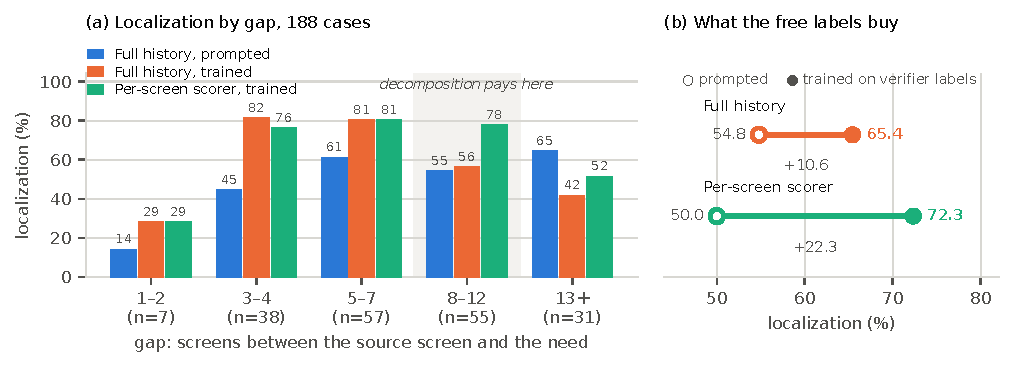
\includegraphics[width=\linewidth]{figures/fig2_results.pdf}
\caption{(a) Localization by gap. The trained variants are level everywhere except at gaps of 8--12 screens, where the per-screen scorer leads by 21.8 points; at 13 or more both fall below prompted full history. (b) What the free labels buy: the same labels lift both architectures, the scorer twice as much. Numbers are in Tables~\ref{tab:main} and~\ref{tab:gap}.}
\label{fig:results}
\end{figure}

\begin{table}[t]
\centering\footnotesize\setlength{\tabcolsep}{4pt}
\caption{Localization (\%) by gap, 188 cases. The trained variants are level except at gaps of 8--12 screens. At gaps of 13 or more both fall below prompted full history.}
\label{tab:gap}
\resizebox{\linewidth}{!}{%
\begin{tabular}{lrrrrr}
\toprule
gap (screens) & $n$ & full history, prompted & full history, trained & \textbf{per-screen scorer} & scorer vs.\ trained FH \\
\midrule
1--2 & 7 & 14.3 & 28.6 & 28.6 & $+$0, 0.48 \\
3--4 & 38 & 44.7 & \textbf{81.6} & 76.3 & $-$2, 0.72 \\
5--7 & 57 & 61.4 & 80.7 & \textbf{80.7} & $+$0, 0.77 \\
8--12 & 55 & 54.5 & 56.4 & \textbf{78.2} & $+$12, \textbf{0.003} \\
13$+$ & 31 & \textbf{64.5} & 41.9 & 51.6 & $+$3, 0.58 \\
\bottomrule
\end{tabular}}
\end{table}

Figure~\ref{fig:results}(a) and Table~\ref{tab:gap} show one band where the architectures diverge. Up to 7 screens back the trained full-history reader matches the scorer, and both improve on prompting by 14 points at gaps of 1--2 ($n=7$, too few to read anything into), 32--37 at 3--4 and 19 at 5--7. At gaps of 8--12 the trained full-history reader stops improving (56.4\%, within 2 points of prompted) while the scorer reaches 78.2\% (net $+12$, \pval{0.003}). This is the band where a single call must weigh a dozen candidates that the task description does not distinguish, and where scoring each screen on its own text pays.

Beyond 12 screens both trained variants fall below prompted full history (41.9\% and 51.6\% against 64.5\%, $n=31$). Training on 188 cases whose gaps have median 5 teaches a prior over distance that misfires at the tail, and the scorer inherits it; the no-distance ablation of Section~\ref{sec:ablation} does not fix the band either. We report this as the method's clearest failure.

\paragraph{Takeaway.} Per-screen scoring is not uniformly better than one call over the history. It wins where the candidate set is large and undifferentiated, and both trained variants lose to prompting at the longest gaps.

\subsection{An external sample confirms the margin over prompting}
\label{sec:ext}
\begin{table}[t]
\centering\footnotesize\setlength{\tabcolsep}{4pt}
\caption{External set: 93 cases from a fourth sample of 400 trajectories, mined after we fixed every design decision. We train each condition on all 188 cross-validated cases and evaluate once. $p$ is against the trained per-screen scorer.}
\label{tab:ext}
\resizebox{\linewidth}{!}{%
\begin{tabular}{lrrrr}
\toprule
condition & localization & $p$ & end-to-end (read with history) & $p$ \\
\midrule
full history, prompted & 59.1 & 0.003 & 23.7 & $<$0.001 \\
screen index, prompted & 37.6 & $<$0.001 & -- & \\
per-screen scorer, prompted & 41.9 & $<$0.001 & -- & \\
full history, trained & 76.3 & 0.63 & 51.6 & 0.62 \\
\textbf{per-screen scorer, trained} & \textbf{79.6} & & \textbf{49.5} & \\
\quad scorer with single-screen read & & & 37.6 & 0.016 \\
\bottomrule
\end{tabular}}
\end{table}

Table~\ref{tab:ext} repeats the comparison on cases that no design decision saw. The scorer localizes 79.6\% against 59.1\% for prompted full history (net $+19$, \pval{0.003}) and 37.6\% for the prompted index (net $+39$, $p<0.001$); the untrained scorer reaches 41.9\%. The trained full-history reader reaches 76.3\%, and the paired test again does not separate it from the scorer (\pval{0.63}), reproducing Section~\ref{sec:main} out of sample. End-to-end, read with history raises accuracy from 23.7\% for prompted full history to 51.6\% for the trained full-history reader (net $+26$, $p<0.001$) and 49.5\% for the scorer, which again the paired test does not separate (net $-2$, \pval{0.62}); the scorer with a single-screen read reaches 37.6\%.

The external needs sit at steps 12--15 (72 cases), 16--19 (19) and 20 or later (2), so this sample tests the mid-range. At 12--15 the scorer localizes 61 of 72 against prompted full history's 42; at 16--19 the two are within one case (12 and 13 of 19).

\paragraph{Takeaway.} On data held out from every design decision, verifier supervision keeps a 20-point margin over prompting, and the two trained variants remain indistinguishable.

\subsection{Ablations and read-stage controls}
\label{sec:ablation}
\begin{table}[t]
\centering\footnotesize\setlength{\tabcolsep}{4pt}
\caption{Left: scorer ablations, localization (\%) on 188 cases, $p$ against the full scorer. Right: read-stage controls, end-to-end (\%) on the same cases, $p$ against marking the scorer's choice.}
\label{tab:abl}
\resizebox{\linewidth}{!}{%
\begin{tabular}{lrr@{\hspace{2em}}lrr}
\toprule
scorer ablation & loc & $p$ & read stage (marked screen) & e2e & $p$ \\
\midrule
full scorer (7B, distance, weight 3) & \textbf{72.3} & & gold source screen marked & \textbf{45.2} & 1.00 \\
no distance in the prompt & 70.7 & 0.61 & \textbf{scorer's choice} & \textbf{44.7} & \\
positive weight 1 & 72.3 & 0.77 & scorer's top two & 45.2 & 1.00 \\
3B base model & 68.1 & 0.22 & most recent screen & 38.8 & 0.10 \\
\quad 3B at $t\ge20$ & \textbf{48.1} & & random earlier screen & 36.7 & 0.018 \\
\bottomrule
\end{tabular}}
\end{table}

Table~\ref{tab:abl} shows the design is insensitive to its prompt and loss settings. Removing the distance from the prompt costs 1.6 points (\pval{0.61}) without rescuing the 13$+$ band, and the positive weight leaves localization at 72.3\%. A 3B base loses 4.2 points overall while gaining 11.1 at $t\ge20$ (48.1\% against 37.0\%).

The read-stage controls bound what marking buys. Marking the gold source screen gives 45.2\% against the scorer's 44.7\%, so the scorer sits at this reader's ceiling, and marking its top two adds nothing. Marking the most recent screen gives 38.8\% and a random earlier screen 36.7\% (\pval{0.018}): repeating any screen accounts for 5--7 of the 13 points over prompted full history, and the chosen screen for the rest.

\subsection{Where the index route stops, and two mandatory filters}
\label{sec:index}
\begin{table}[t]
\centering\footnotesize\setlength{\tabcolsep}{4pt}
\caption{Short set ($n=85$), localization (\%). The screen index's writer cannot pass full history, and an oracle that rewrites only the source screen's line reaches full-history level and no higher.}
\label{tab:index}
\resizebox{\linewidth}{!}{%
\begin{tabular}{lr@{\hspace{2em}}lr}
\toprule
condition & loc & writer variant / oracle & loc \\
\midrule
no history (end-to-end 2.4) & n/a & writer trained with DPO on the same 85 cases & 45.9 \\
full history, prompted & 65.9 & writer forced to a two-field format & 47.1 \\
per-screen summary & 23.5 & writer allowed to copy values & 49.4 \\
screen index, prompt-only & 49.4 & writer: three lines per screen & 43.5 \\
BM25, task $+$ current screen as query & 10.6 & writer: retrieval prompt, sampled, every screen & 44.7 \\
BM25, gold text as query & 92.9 & oracle: source line replaced by 1 of 5 sampled lines & 58.8--65.9 \\
\textbf{per-screen scorer, trained} & \textbf{77.6} & oracle: best of the five sampled lines per case & 76.5 \\
\bottomrule
\end{tabular}}
\end{table}

We built the screen index first; Table~\ref{tab:index} records why we left it. The prompt-only index localizes 49.4\% against 65.9\% for full history (\pval{0.035}). We trained its writer with direct preference optimization~\citep{dpo} on 224 preference pairs built from the same 85 cases that we score it on, a choice that favors it. It localizes 45.9\%, and four prompt variants stay between 43.5\% and 49.4\%. An oracle that replaces only the source screen's line with one of five lines sampled at temperature 0.9 gives 58.8--65.9\%, level with full history ($p\ge0.36$). The best of the five per case gives 76.5\%, but 64\% of cases are insensitive to which line it uses, so that gain is redundancy no single writer realizes. BM25 localizes 92.9\% with the gold text as query and 10.6\% with what the agent actually knows: the difficulty is deciding what to look for, which a 32-token line does not ease.

\paragraph{Two filters move conclusions more than any method.} \emph{Earliest-source scoring} labels only the earliest screen that contains the text, but 47\% of short-set cases have two or more; scoring any valid screen lifts the index 15.3 points and full history 11.8. \emph{Current-screen leakage} admits cases whose answer is also on the current screen (28\% of short-set and 58\% of long-set candidates). On the 127 unfiltered long-set cases a rule that reads only the two previous screens beats full history by 17.3 points (\pval{0.010}); on the 53 clean ones it loses by 22.7 (\pval{0.019}). We found this by noticing that the rule's localization gain did not move end-to-end accuracy, and we retracted the result. Both filters are one condition each: at mining time the answer must be absent from the current screen's OCR, and at scoring time any screen whose OCR contains the answer counts as correct.

\subsection{Limits}
\label{sec:limits}
Gaps of 13 or more screens are the method's clearest failure: both trained variants fall below prompted full history and no ablation recovers the band. At $t\ge20$ ($n=27$) the 7B scorer matches prompted full history (37.0\%), while the trained full-history reader reaches 44.4\% and a 3B scorer 48.1\%, so neither our preferred variant nor its size is the right choice at the longest histories. We cross-validate on one dataset with one OCR engine, and the external set comes from the same corpus. The training labels and the localization metric are the same substring check, so training points the scorer at the metric we score it on; a spot check of 20 verified cases found that every labeled screen did show the needed text, and that in 5 of them the agent had typed the text itself earlier (a search query or a note title), which makes the need weaker in those 5. Each condition is a single training run, so our paired tests account for case-level variance only. The scorer's maximum probability predicts whether its localization is correct with an area under the ROC curve of 0.768; falling back to prompted full history below 0.5 raises localization to 75.0\%, which we report but do not use.

\section{Related work}

\paragraph{Memory for GUI agents.} AutoDroid~\citep{autodroid}, AppAgent~\citep{appagent}, Agent Workflow Memory~\citep{awm}, Synapse~\citep{synapse} and the tips and shortcuts of Mobile-Agent-E~\citep{mobileagente} store knowledge that transfers across episodes; they answer how to do a task, not what this episode showed. Mobile-Agent-E's note-taker and GUI-Rise's rolling summary~\citep{guirise} write notes at observation time, before the agent knows what it will need, which is exactly the regime in which the needed text is inconspicuous (median rank 13 of 33 elements). PAL-UI~\citep{palui} is the closest prior work: it trains a vision agent to look back at chosen frames, supervised by 8.6K curated step-level instructions. Our verifier replaces that supervision with a substring test over OCR text, so the training set grows with any corpus of trajectories that records typed text.

\paragraph{Gist-and-lookup and learned retrieval.} ReadAgent~\citep{readagent}, MemGPT~\citep{memgpt} and Generative Agents~\citep{generativeagents} retrieve from short per-item lines or scored memory streams. Document expansion~\citep{doc2query} trains the \emph{writer} of those lines from downstream success, and tool self-supervision~\citep{toolformer} filters tool calls by whether they reduce later loss. We train the retriever instead of the writer, after finding that the writer's ceiling is the screen itself (Section~\ref{sec:index}), and our filter is an exact substring check rather than a loss proxy.

\paragraph{Long-context evaluation.} Lost-in-the-middle~\citep{lostmiddle} and RULER~\citep{ruler} show that models use long contexts unevenly and that synthetic needle tasks overstate usable length. Ours is a needle task on real screens with contexts of 1--5K tokens, short enough that full history still helps. The two filters of Section~\ref{sec:index} are specific to needles mined from trajectories, where a needle can recur and can sit on the current screen.

\section{Code and experiment running snippets}
\label{sec:code}
All code, every result file, and the scripts that draw both figures are at
\url{https://github.com/WMSlalalala/verifier-supervised-lookback}. The repository README documents
each file, class and function, states which parts we wrote ourselves (all of \texttt{src/}; the
external dependencies are EasyOCR, \texttt{transformers}, \texttt{peft} and the Qwen2.5 models), and
lists the commands below. The DPO loss, the McNemar test, the BM25 scorer and the trajectory-grouped
fold splitter are hand-written rather than taken from a library.

\paragraph{Build the dataset and the labels.} \texttt{sample\_more.py} picks trajectories and downloads
their screenshots, \texttt{ocr\_shots.py} runs EasyOCR over them, and \texttt{verify\_more.py} applies
the verifier, writing both the cases and the label sets.
\begin{lstlisting}[language=bash]
MINLEN=16 MINT=12 N=400 python src/sample_more.py  # 400 trajectories
python src/ocr_shots.py          # resumable; appends to parse_odyssey.jsonl
python src/verify_more.py        # -> cases_more.json + valid_screens_more.json
python src/build_scorer_data.py  # -> 188 cases, 2,861 pairs, 5 folds
\end{lstlisting}

\paragraph{Train both instantiations and the ablations.} \texttt{FOLD} selects the held-out fold,
\texttt{TAG} names the run, and \texttt{NODIST}, \texttt{POSW} and \texttt{MODEL} drive the three
ablations. One fold takes 13--27 minutes on one 48GB GPU.
\begin{lstlisting}[language=bash]
FOLDS="0 1 2 3 4"; M3B=Qwen/Qwen2.5-3B-Instruct
for f in $FOLDS; do FOLD=$f python src/train_scorer.py;   done  # scorer
for f in $FOLDS; do FOLD=$f python src/train_fullhist.py; done  # full history
python src/score_untrained.py                      # same prompt, no adapter
for f in $FOLDS; do FOLD=$f TAG=_nodist NODIST=1 python src/train_scorer.py; done
for f in $FOLDS; do FOLD=$f TAG=_posw1  POSW=1   python src/train_scorer.py; done
for f in $FOLDS; do FOLD=$f TAG=_3B MODEL=$M3B   python src/train_scorer.py; done
\end{lstlisting}

\paragraph{Read stage, its controls, and the prompted baselines.}
\begin{lstlisting}[language=bash]
SRC=trained HIST=1 python src/read_scorer.py     # read with history
SRC=trained        python src/read_scorer.py     # single-screen read
for m in gold recent random top2; do
  SRC=trained HIST=1 MARK=$m python src/read_scorer.py            # controls
done
CASES=long MODE=B python src/eval_long.py        # full history, prompted
CASES=long MODE=D python src/eval_long.py        # screen index, prompted
\end{lstlisting}

\paragraph{External set: train once on all 188, evaluate once.}
\begin{lstlisting}[language=bash]
FOLD=ext python src/train_scorer.py
FOLD=ext python src/train_fullhist.py
SRC=trained SET=_more HIST=1 python src/read_scorer.py
\end{lstlisting}

\paragraph{Reproduce every table and figure.} \texttt{analyze\_all.py} reads the committed result
files and prints Tables~\ref{tab:main}--\ref{tab:abl} with their paired tests; it needs no GPU.
\begin{lstlisting}[language=bash]
python src/analyze_all.py
python figures/make_fig1.py && python figures/make_fig2.py
\end{lstlisting}

\paragraph{Running on shared GPUs.} The \texttt{run\_*.sh} drivers wrap the commands above. Each
waits for a GPU with enough free memory before starting a job (\texttt{pick()}), skips any stage
whose output already exists, and retries on failure, so a run that is interrupted or evicted resumes
where it stopped. This mattered: one stage of our experiments was evicted mid-run by a co-tenant job
and resumed from the completed folds.

\section{Conclusion}
The verifier that defines a delayed information need also labels which earlier screens answer it, so
look-back trains on any corpus of agent trajectories without a person labeling anything. That
supervision is the lever: it lifts a one-call full-history reader by 10.6 localization points and a
per-screen scorer by 22.3, and it reverses which of the two architectures is better. The
decomposition buys a further 6.9 points of localization and 2.1 end-to-end, neither of which a paired
test separates, and 21.8 points at gaps of 8--12 screens, where one call must weigh many
undifferentiated candidates. On a fourth sample held out from every design decision, both trained
variants keep a 17--20 point localization margin over prompting and reach 49.5\% and 51.6\%
end-to-end against 23.7\%, remaining indistinguishable from each other. Gaps of 13 or more screens
stay open: both trained variants fall below prompting there, and a 3B scorer is the only variant that
improves the latest needs. We also report two evaluation filters without which these measurements are
not meaningful, one of which forced us to retract an earlier result of our own.

{\small\bibliographystyle{plainnat}\bibliography{refs}}
\end{document}
